\documentclass[]{rptuseminar}

% Specify that the source file has UTF8 encoding
\usepackage[utf8]{inputenc}
% Set up the document font; font encoding (here T1) has to fit the used font.
\usepackage[T1]{fontenc}
\usepackage{lmodern}

% Load language spec
\usepackage[american]{babel}
% German article --> ngerman (n for »neue deutsche Rechtschreibung«)
% British English --> english

% Ffor bibliography and \cite
\usepackage{cite}

% AMS extensions for math typesetting
\usepackage[intlimits]{mathtools}
\usepackage{amssymb}
% ... there are many more ...


% Load \todo command for notes
\usepackage{todonotes}
% Sebastian's favorite command for large inline todonotes
% Caveat: does not work well with \listoftodos
\newcommand\todoin[2][]{\todo[inline, caption={2do}, #1]{
		\begin{minipage}{\linewidth-1em}\noindent\relax#2\end{minipage}}}

% Load \includegraphics command for including pictures (pdf or png highly recommended)
\usepackage{graphicx}

% Typeset source/pseudo code
\usepackage{listings}

% Load TikZ library for creating graphics
% Using the PGF/TikZ manual and/or tex.stackexchange.com is highly adviced.
\usepackage{tikz}
% Load tikz libraries needed below (see the manual for a full list)
\usetikzlibrary{automata,positioning}

% Load \url command for easier hyperlinks without special link text
\usepackage{url}

% Load support for links in pdfs
\usepackage{hyperref}

% Defines default styling for code listings
% \definecolor{pink}{rgb}{}
\definecolor{green_ulises}{rgb}{0.2,0.75,0}
\lstdefinelanguage{smtlib2} {
  morekeywords={set-logic, declare-const, assert, check-sat, get-model},
  sensitive=true,
  morecomment=[l]{;},
  morestring=[b]"
}

\lstset{%
  columns=flexible,
  keepspaces=true,
  tabsize=3,
  basicstyle={\fontfamily{tx}\ttfamily\small},
  stringstyle=\color{green_ulises},
  commentstyle=\color{black!80}
  identifierstyle=\slshape{},
  keywordstyle=\bfseries,
  numberstyle=\small\color{pink},
  backgroundcolor=\color{gray!5},
  numberblanklines=false,
  inputencoding={utf8},
  showstringspaces=false,
  belowskip=-1mm,
  escapeinside={//*}{\^^M} % Allow to set labels and the like in comments
}

% Defines a custom environment for indented shell commands
\newenvironment{displayshellcommand}{%
	\begin{quote}%
	\ttfamily%
}{%
	\end{quote}%
}

%%%%%%%%%%%%%%%%
\lstnewenvironment{haskell}{
  \vspace{1em}%
  \lstset{
    language=Haskell,
    columns=flexible,
    keepspaces=true,
    tabsize=3,
    basicstyle={\fontfamily{tx}\ttfamily\small},
    stringstyle=\color{green_ulises},
    commentstyle=\color{black!80},
    identifierstyle=\slshape{},
    keywordstyle=\bfseries,
    numberstyle=\small\color{pink},
    backgroundcolor=\color{gray!5},
    numberblanklines=false,
    inputencoding={utf8},
    belowskip=-1mm,
    escapeinside={//*}{\^^M} % Allow to set labels and the like in comments
  }
}{
  \vspace{1em}
}%%%%%%%%%%%%%%%%%%%%%%%%%%%%%%%%%%%%%%%%%%%%%%%%%%%%%%%%%%%%%%%

\title{\textsc{Liquid}{H}\textsc{askell}}
\event{Seminar: Programming Languages in Winter term 2024/2025}
\author{Mehran Shahidi, Saba Safarnezhad
  \institute{Rheinland-Pfälzische Technische Universität Kaiserslautern-Landau, Department of Computer Science}}

%%%%%%%%%%%%%%%%%%%%%%%%%%%%%%%%%%%%%%%%%%%%%%%%%%%%%%%%%%%%%%%%%%%%%%%%%%%%%%%
\begin{document}
%%%%%%%%%%%%%%%%%%%%%%%%%%%%%%%%%%%%%%%%%%%%%%%%%%%%%%%%%%%%%%%%%%%%%%%%%%%%%%%

\maketitle

%%%%%%%%%%%%%%%%%%%%%%%%%%%%%%%%%%%%%%%%%%%%%%%%%%%%%%%%%%%%%%%%%%%%%%%%%%%%%%%

\begin{abstract}
  This report gives a brief overview of \texttt{LiquidHaskell}, a tool that extends Haskell with refinement types. 
  Refinement types are types that extends expressiveness of Haskell types systems by providing predicates that can verify
  invarients of the program. This report explains briefly how SMT solvers leveraged by \texttt{LiquidHaskell} and 
  how to use \texttt{LiquidHaskell} by providing some examples. Finally, we discuss the limitations of \texttt{LiquidHaskell} and compare it with other tools.
\end{abstract}

%%%%%%%%%%%%%%%%%%%%%%%%%%%%%%%%%%%%%%%%%%%%%%%%%%%%%%%%%%%%%%%%%%%%%%%%%%%%%%

\section{Introduction}
\label{sec:introduction}
Programming verification is an important step in software development. It is the process of
verifying that a program behaves as expected. There has been a lot of research in this 
area and many tools have been developed. 
Type safety is one of the important features of programming languages that helps to prevent runtime errors.
Despite catching many errors at compile time, type systems are not powerful enough to catch all the errors.
On the other hand, testing is another way to verify the program, but it is not always possible to test all the possible inputs.
Consider the following example:

\begin{haskell}
  average    :: [Int] -> Int
  average xs = sum xs `div` length xs
\end{haskell}

The example above is a simple function that calculates the average of a list of integers. This can be a source of runtime
error if the list is empty. While this can be caught by testing, it is not always possible to test all the possible inputs.
Another way to verify the program is to use program verification tools. These tools use mathematical logic to check the program.
One of such tools that is used in Haskell programming language is \texttt{LiquidHaskell}. \texttt{LiquidHaskell} 
(\texttt{LiquidHaskell}) extends Haskell with refinement types which are types that extend the expressiveness of Haskell.
With refinement types, we can provide invariant that the program should satisfy \cite{jhala_programming_2020}. 

In this report, after a short backgrouund on program verfication using SMT in section \ref{sec:background}, we will explain 
how \texttt{LiquidHaskell} works and how it uses SMT solvers to 
verify the program in section \ref{sec:lh}. Then in section \ref{sec:example} we will provide some examples how to use 
\texttt{LiquidHaskell} to verify persistent stack. Finally in section \ref{sec:conclusions} we 
discuss the limiations of \texttt{LiquidHaskell} and compare it with other tools.

% E.~g.~ 
% ``quoting'' is done by using two backticks and two single quotes

\section{Overview}
\label{sec:background}

\subsection{Type Systems and Program Verification}
Programming verification ensures that software behaves as expected by using formal methods. 
One common approach is type safety, which helps catch errors at compile time. 
However, traditional type systems in functional languages like Haskell often lack expressiveness 
to specify and enforce complex program properties statically \cite{jhala_programming_2020}. 
While testing is another method for verification, 
it is impractical to cover all possible inputs, especially in large-scale applications.

\subsection{Refinement Types}
Refinement types extend conventional type systems by attaching logical predicates to types. 
This allows for more precise specifications of program invariants. 
For instance, in \texttt{LiquidHaskell}, a type annotation ensures that a function always receives a positive integer:

\begin{haskell}
{-@ incr :: Pos -> Pos @-}
incr :: Int -> Int
incr x = x + 1
\end{haskell}

Here, \texttt{Pos} is a refinement type that guarantees the argument and result are strictly positive integers. 
Unlike standard type systems, refinement types use logical constraints to enable static program verification.
\cite{vazou_refinement_2014}.

\subsection{SMT Solvers}
Satisfiability Modulo Theories (SMT) solvers extend SAT solvers by incorporating various 
mathematical theories (e.g., arithmetic, arrays, lists). These solvers determine the 
satisfiability of logical formulas with complex constraints \cite{clarke_satisfiability_2018}. 
A common SMT solver used in verification is Z3, which supports multiple theories and decision procedures.

For example, given the constraints:

\begin{equation}
x + y \leq 10 \quad \text{and} \quad x = y - 7
\end{equation}

An SMT solver can determine whether a valid assignment exists for \(x\) and \(y\).

\subsection{\texttt{LiquidHaskell} and SMT}
\texttt{LiquidHaskell} integrates refinement types with SMT solvers to perform automated verification. 
It encodes refinement predicates as logical formulas and delegates their satisfiability checking to an SMT solver like Z3 
\cite{vazou_refinement_2014}. 

For example, a refined list function can ensure non-empty lists:

\begin{haskell}
{-@ tail :: {v:[a] | 0 < len v} -> a @-}
tail :: [a] -> a
tail (x:_) = x
\end{haskell}

This ensures that \texttt{tail} is only applied to non-empty lists, preventing runtime errors. 
The SMT solver checks that all function applications adhere to their specifications, 
making \texttt{LiquidHaskell} a powerful tool for static verification.

\subsection{SMT Solvers}
SMT (Satisfiability Modulo Theories) solvers are tools that can check the satisfiability of logical formulas in a specific theory.
SMT solvers extend the concept of SAT solvers by adding theories (e.g., the theory of equality, 
of integer numbers, of real numbers, of arrays, of lists, and so on) to the boolean logic \cite{clarke_satisfiability_2018}.
While SAT solvers can only check the satisfiability of boolean formulas, SMT solvers can check the satisfiability of formulas 
that contain variables from different theories. 
As an example, consider the following formula:

\begin{equation}
  \varphi = (x \lor y) \land (\lnot x \lor z)
\end{equation}

A SAT solver can check the satisfiability of the formula \(\varphi\) by checking if there is an assignment for the variables \(x, y, z\).
For instance, \(x = true, y = false, z = true\) is an assignment that makes \(\varphi\) \(true\). 

On the other hand, SMT solvers can check the satisfiability of formulas that contain variables that required arithmetic theory as following formula:

\begin{equation}
  x + y \leq 10 \quad and \quad x = y - 7
\end{equation}

\subsection{Z3 SMT Solvers}
\subsubsection*{Overall System Architecture of Z3}
The overall system architecture of Z3 is aimed at efficiently solving Satisfiability Modulo Theories (SMT) problems. Here's a detailed breakdown of the major components and their interactions:

 \begin{figure}[ht]
  \begin{center}
    \fbox{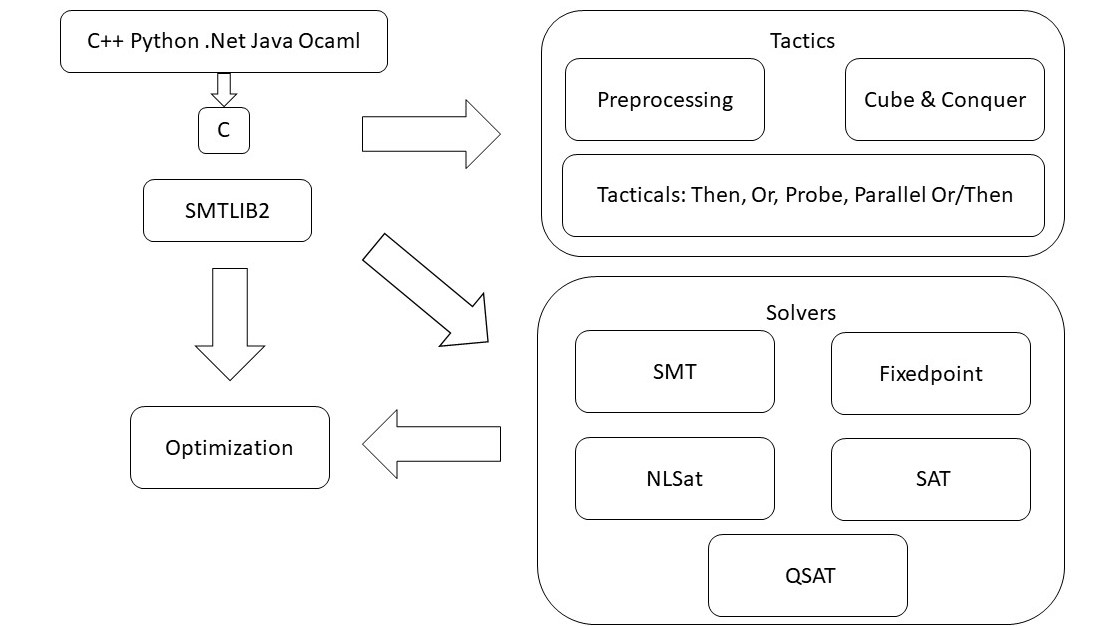
\includegraphics[width=.9\linewidth]{SMT}}%
    % fbox for "framed box"
  \end{center}
  \caption{%
     Overall system architecture of Z3
    \cite{nikolaj_bjorner_programming_nodate}
  }
  \label{fig:scholar} % NOTE: \label must appear after \caption
\end{figure}

\subsubsection{Interfaces to Z3}
Z3 can be interacted with using SMT-LIB2 scripts supplied as text files or through a pipe.
Besides this, high-level programming languages can make API calls to Z3, which are proxies
for calls over a C-based API \cite{nikolaj_bjorner_programming_nodate}.

\subsubsection{Logical Formulas}
Z3 accepts logical formulas built from atomic variables and logical connectives, which can include symbols defined by various theories.
These formulas use basic building blocks like Boolean variables, integers, and reals, combined with logical operators such as
\texttt{And}, \texttt{Or}, \texttt{Not}, \texttt{Implies}, and \texttt{Xor}. Z3 handles complex logical expressions by
integrating symbols from multiple theories, such as arrays and arithmetic, allowing it to model a wide range of problems.
The formulas generally follow the SMT-LIB2 standard, ensuring interoperability between different SMT solvers. 
This versatility makes Z3 a powerful tool for solving diverse logical problems efficiently \cite{nikolaj_bjorner_programming_nodate}.

\subsubsection{Theories}
Z3 supports multiple theories, including Equality and Uninterpreted Functions (EUF), Arithmetic (both linear and non-linear),
Arrays, Bit-Vectors, Algebraic Datatypes, Sequences, and Strings. Each theory has specialized decision procedures for solving
related formulas \cite{nikolaj_bjorner_programming_nodate}.


\subsubsection{Solver}
Z3 provides services for deciding the satisfiability of formulas. This includes handling incrementality, scopes, assumptions, 
cores, models, and other methods like statistics, proofs, and retrieving solver state. Specialized solvers are included for 
different types of problems \cite{nikolaj_bjorner_programming_nodate}.

\subsubsection*{SMT Solver}
The SMT solver in Z3 is a general-purpose solver that integrates various theories to decide the satisfiability of logical formulas. 
It uses the CDCL(T) architecture, which combines Conflict-Driven Clause Learning (CDCL) with theory solvers \cite{nikolaj_bjorner_programming_nodate}.

\subsubsection*{Fixedpoint Solver}
The Fixedpoint solver in Z3 is used for reasoning about recursive definitions and fixed-point computations. 
It includes a Datalog engine and supports relational algebra and Property Directed Reachability (PDR) algorithms \cite{nikolaj_bjorner_programming_nodate} 

\subsubsection*{NLSat Solver}
The NLSat solver is specialized for non-linear arithmetic problems. 
It uses a combination of algebraic methods and SAT solving techniques to handle polynomial constraints \cite{nikolaj_bjorner_programming_nodate}.

\subsubsection*{SAT Solver}
The SAT solver in Z3 is designed for propositional logic problems. It uses advanced techniques like in-processing 
and co-processing to efficiently solve Boolean satisfiability problems \cite{nikolaj_bjorner_programming_nodate}.

\subsubsection*{QSAT Solver}
The QSAT solver handles quantified Boolean formulas (QBF). It extends the capabilities of the SAT solver to deal with quantifiers, 
providing solutions for more complex logical problems \cite{nikolaj_bjorner_programming_nodate}.


\subsubsection{Tactics}
Tactics in Z3 are used for preprocessing, formula simplification, and the generation of sub-goals. they
are essential to decompose complex problems into relatively simple fragments. The preprocess tactics simplify the input formulae before they are fed into the main solver. It can include heuristics such as the propagation of constants, arithmetic simplification, and removal of redundant constraints. The Cube and Conquer tactic is used to split the search space into smaller sub-problems. (cubes) that can be solved independently. This is a very useful scheme for parallel solving
and the sum time required to solve, it greatly shortens. Tacticals are combiners which make composition of multiple tactics \cite{nikolaj_bjorner_programming_nodate}.
\subsubsection{Optimization}
Z3 allows the use of optimization services along with user-defined problems in order to study the satisfiability of the problem while maximizing or minimizing objective functions. This applies to those problems which require solutions that are to be optimized under given constraints \cite{nikolaj_bjorner_programming_nodate}.

\subsubsection{Applications and Example of Z3}
Software analysis verification and symbolic execution along with software analysis verification rely heavily on making use of the Z3 platform. Z3 operates through SMT-LIB2 scripts for textual logical problem inputs as well as program application interfaces using Python fundamental sources and C++ constructs and OCaml programming code. Both Z3 users prefer the Python API because of its straightforward nature and SMT-LIB2 stands out for presenting logical problems with predefined logics including arithmetic, arrays and bit-vectors.
\vspace{1em}

To be sure, consider \ref{eq:example-sat} and its satisfiability problem,
we are wondering is there a value assignment of Boolean variables Tie, Shirt,
such that three clauses conjuction :


\begin{equation}
  \label{eq:example-sat}
  (Tie \lor Shirt) \land (\lnot Tie \lor Shirt) \land (\lnot Tie \lor \lnot Shirt)
\end{equation}

Formula \ref{eq:example-sat}  can be solved in SMTLIB2 as following code:

\begin{figure}[ht]
  \begin{lstlisting} [language=SMTlIB2]
    (set-logic QF_UF)
    (declare-const Tie Bool)
    (declare-const Shirt Bool)
    (assert (or Tie Shirt))
    (assert (or (not Tie) Shirt))
    (assert (or (not Tie) (not Shirt)))
    (check-sat)
    (get-model)
  \end{lstlisting}
  \end{figure}

  When we run this, Z3 responds:
\begin{lstlisting} [language=SMTlIB2]
 sat
 (model
   (define-fun Tie () Bool false)
   (define-fun Shirt () Bool true)
 )
\end{lstlisting}
\vspace{1em}

  This SMT-LIB2 script sets up the problem, declares the variables, asserts the constraints, checks for satisfiability, and retrieves the model, just like the Python code does for Formula \ref{eq:example-sat}  with z3 in the following example.

\begin{figure}[ht]
\begin{lstlisting}[language=Python]
  from z3 import Bools, Solver, Or, Not
  Tie, Shirt = Bools('Tie Shirt')
  s = Solver()
  s.add(Or(Tie, Shirt),
        Or(Not(Tie), Shirt),
        Or(Not(Tie), Not(Shirt)))
  print(s.check())
  print(s.model())
\end{lstlisting}
\end{figure}

\vspace{1em}
The output of the code is:
\begin{lstlisting}[language=Python]
sat

[Tie = False, Shirt = True]
\end{lstlisting}
\vspace{1em}


When calling s.check(), the solver determines that the assertions are satisfiable (sat)—meaning there is a way to assign values to Tie and Shirt that makes all the conditions true. One possible solution is Tie = false and Shirt = true, which can be retrieved using s.model().
\vspace{1em}



The next example shows how Z3 reasons across multiple mathematical theories such as array theory, arithmetic, and uninterpreted functions. Z3's API analyzes the following Python snippet:


\begin{lstlisting}[language=Python]
Z = IntSort()
f = Function('f', Z, Z)
x, y, z = Ints('x y z')
A = Array('A', Z, Z)
fml = Implies(x + 2 == y, f(Store(A, x, 3)[y - 2]) == f(y - x + 1))
solve(Not(fml))

unsat
\end{lstlisting}



\paragraph{Theories Involved}
The integrated theories enabling this reasoning are:

\begin{itemize}
    \item \textbf{Linear Integer Arithmetic (LIA)}: Handles integer constraints:
    \begin{equation*}
        x + 2 = y \quad \text{and} \quad y - x + 1
    \end{equation*}
    
    \item \textbf{Array Theory}: Manages array operations through \texttt{Store} and select operators:
    \begin{equation*}
        \texttt{Store}(A, x, 3)[y - 2] \equiv \text{ite}(y - 2 = x, 3, A[y - 2])
    \end{equation*}
    where \text{ite} denotes the if-then-else operator.
    
    \item \textbf{Uninterpreted Functions}: Treats function $f$ as a black box respecting functional consistency:
    \begin{equation*}
        \forall a, b: (a = b) \implies (f(a) = f(b))
    \end{equation*}
\end{itemize}

This example illustrates Z3's theory combination mechanism, which:
\begin{itemize}
    \item Ensures coherence across different mathematical domains
    \item Handles cross-theory constraints (e.g., array indices as arithmetic expressions)
    \item Enables verification of systems with mixed abstractions (memory, arithmetic, and black-box components)
\end{itemize}

This capability makes Z3 particularly useful for software verification, as real-world programs inherently integrate these concepts \cite{nikolaj_bjorner_programming_nodate}.
\section{Working with \texttt{LiquidHaskell}}
\label{sec:lh}
\texttt{LiquidHaskell} is a tool that extends Haskell with refinement types. Refinement types enhance 
the expressiveness of Haskell types systems by providing predicates that can verify invariants of the program \cite{vazou_refinement_2014}.
In this section, we will explain how \texttt{LiquidHaskell} works.
\texttt{LiquidHaskell} is available as a GHC plugin. To use it, you need to add its dependencies to the cabal file as following \cite{noauthor_ucsd-progsyslh-plugin-demo_2024}:

\vspace{1em}
\begin{lstlisting}
 cabal-version: 1.12

 name:           lh-plugin-demo
 version:        0.1.0.0
 ...
 ...
   build-depends:
       liquid-prelude,
       liquid-vector,
       liquidhaskell,
       base,
       containers,
       vector
   default-language: Haskell2010
   ghc-options:  -fplugin=LiquidHaskell
\end{lstlisting}
\vspace{1em}

By adding this dependency, \texttt{LiquidHaskell} can now check your program at compile time or via code linter in your IDE of choice.
In the following sections, we will explain how to use \texttt{LiquidHaskell} to verify the program.
\subsection{Type Refinement}
Refinement types allow to constrain the type of the variables by adding predicates to the types 
\cite{jhala_programming_2020}. For example, we can define natural numbers as follows:

\begin{haskell}
 {-@ type Nat = {v:Int | 0 <= v} @-}
\end{haskell}

Now if you configure your IDE to use Haskell LSP, it will show the following error if you try to assign a negative number
to a variable of type Nat.

\begin{haskell}
 {-@ x :: Nat @-}
 x = -1
 >>> typecheck: Liquid Type Mismatch
   .
   The inferred type
     VV : {v : GHC.Types.Int | v == GHC.Num.negate (GHC.Types.I# 1)
                               && v == (-GHC.Types.I# 1)}
   .
   is not a subtype of the required type
     VV : {VV##493 : GHC.Types.Int | VV##493 >= 0}
   .
   Constraint id 2
\end{haskell}

The error message shows that the inferred type of the variable x is not a subtype of the required type.

Using refinement types, one can define pre-conditions and post-conditions of the functions\cite{jhala_programming_2020}. 
For example, consider the following function:

\begin{haskell}
 tail :: [a] -> [a]
 tail (_:xs) = xs
 tail [] = error "tail: empty list"
\end{haskell}

The function defined above is a partial function because it does not handle the case when the list is empty. 
 Typical Haskell types only allow the introduction of the Maybe type, which postpones error 
 handling to another part of the program \cite{jhala_programming_2020}. Using refinement types, we can define the type of tail function as follows:

\begin{haskell}
 {-@ tail :: {v:[a] | 0 < len v} -> a @-}
 tail :: [a] -> [a]
 tail (x:_) = x
\end{haskell}

Now our function is a total function as it doesn't allow the non-empty list to be passed to the \textit{tail}. However, it can't 
check the following case.

\begin{haskell}
 x :: [Int]
 x = tail (tail [1, 2])
\end{haskell}

When calling functions, \texttt{LiquidHaskell} won't look into the body of the function to see if the first application of \textit{tail} gives the valid non-empty list to the second \textit{tail}.
To allow \texttt{LiquidHaskell} consider the above example as safe, we need to also specify the post-condition for our function as following:

\begin{haskell}
 {-@ tail :: xs: {v:[a] | 0 < len v} -> {v:[a] | len v == len xs - 1} @-}
 tail :: [a] -> [a]
 tail (x:_) = x
\end{haskell}

\subsection{Refined Data Types}
In the above examples, we saw how refinements of input and output of function allow us to have stronger arguments about our program. 
We can take this further by refining the data types. Consider the following example \cite{jhala_programming_2020}:

\begin{haskell}
  data Slist a = Slist { size :: Int, elems :: [a] }

  {-@ data Slist a = Slist { size :: Nat, elems :: {v:[a] | len v == size} } @-}
\end{haskell}

This refined \textit{Slist} data type ensures the stored `size` always matches the length of the `elems` list, 
as formalized in the refinement annotation \cite{jhala_programming_2020}. 
This ensures that the size of the list is always correct.

The only thing that is missing is the definition of \textit{len}. Fortunately, this function has already reflected by
\texttt{LiquidHaskell}. In the following section, we show how can we use reflection or measure directives to define and execute any user-defined Haskell function in the refinement logic and
reason about them.

\subsection{Lifting Functions to the Refinement Logic}
When our programs become more complex, we need to define our own functions in the refinement logic and reason about
a function within another function. Refinement Reflection allows deep specification and verification by 
reflecting the code implementing a Haskell function into the function’s output refinement type \cite{niki_blog_2016}.
There are two ways to define and reason about a function in the refinement logic: \texttt{reflection} and \texttt{measure}. 

\texttt{Measure} can be used on a function with one argument that is pattern-matched in the function body. Then,
\texttt{LiquidHaskell} copies the function to the refinement logic, adds a refinement type to the constructor of the function's argument, and emits inferred global
invariants related to the refinement. Consider the following example:

\begin{haskell}
data Bag a = Bag { toMap :: M.Map a Int } deriving Eq
{-@ measure bag @-}
{-@ bag :: Ord a => List a -> Bag a @-}
bag :: (Ord a) => List a -> Bag a
bag Emp = B.empty
bag (Cons x xs) = B.put x (bag xs)
\end{haskell}

This code add the bag refinement type to the List data type. The \texttt{measure} directive is used to define the \texttt{bag} function,
which is then copied to the refinement logic. It means that now the type of list constructors would have:

\begin{haskell}
Nil  :: {v:List a | bag v = B.empty}
Cons :: x:a -> l:List a -> {v:List a | bag v = B.put x (bag l)}
\end{haskell}

So then we can use the \texttt{bag} function in the refinement logic to reason about the program. 
For instance, in the following example, we can use the \texttt{bag} function to reason about the program:

\begin{haskell}
{-@ equalBagExample1 :: { bag(Cons 1 (Cons 3 Emp)) ==  bag( Cons 2 Emp) } @-}

>>    VV : {v : () | v == GHC.Tuple.Prim.()}
>>    .
>>    is not a subtype of the required type
>>      VV : {VV##2465 : () | bag (Cons 1 (Cons 3 Emp)) == bag (Cons 2 Emp)}
\end{haskell}

The $\{x = y\}$ is shorthand for $\{ v : () \mid x = y \}$, where $x$ and $y$ are expressions.
Note that equality for bags is defined as the equality of the underlying maps that already have a built-in equality function.
\texttt{LiquidHaskell} can reason about the equality of bags by using the equality of the underlying maps and issuing a type error if the bags are not equal.
If we define multiple measures for the same data type the refinements are conjoined together \cite{niki_lecture_2024}.



Reflection is another useful feature that allows the user to define a function in the refinement logic, providing
the SMT solver with the function's behavior \cite{vazou_refinement_2018}. 
This has the advantage of allowing the user to define a function that is not pattern-matched in the function body.
Additionally, with the use of a library of combinators provided by \texttt{LiquidHaskell}, we can leverage the existing programming constructs to 
prove the correctness of the program and use the principle of propositions-as-types (known as Curry-Howard isomorphism)\cite{vazou_refinement_2018}\cite{wadler_propositions_2015}.

\begin{haskell}
{-@ infixr ++ @-}
{-@ reflect ++ @-}

{-@ (++) :: xs:[a] -> ys:[a] -> { zs:[a] | len zs == len xs + len ys } @-}
(++) :: [a] -> [a] -> [a]
[] ++ ys = ys
(x : xs) ++ ys = x : (xs ++ ys)
\end{haskell}

The \texttt{++} function is defined in the refinement logic using the \texttt{reflect} directive.
Now we can use the \texttt{++} function in the refinement logic to reason about the program.
In the following subsection, we will show how to use \texttt{LiquidHaskell} to verify that  the \texttt{++} function is associative.

\subsection{Verification}
\texttt{LiquidHaskell} allows structure proofs to follow the style of calculational or equational reasoning popularized in classic texts
and implemented in proof assistants like Coq and Agda . \texttt{LiquidHaskell} is equipped with a family of equation combinators
for logical operators in the theory QF-UFLIA \cite{vazou_refinement_2018}.
In the following example, we show how to use \texttt{LiquidHaskell} to verify that the \texttt{++} function is associative:

\begin{haskell}
{-@ assoc :: xs:[a] -> ys:[a] -> zs:[a] 
  -> { v: () | (xs ++ ys) ++ zs = xs ++ (ys ++ zs) } @-}
assoc :: [a] -> [a] -> [a] -> ()
assoc [] ys zs =
  ([] ++ ys)
    ++ zs
    === ys
    ++ zs
    === []
    ++ (ys ++ zs)
    *** QED

assoc (x : xs) ys zs =
  ((x : xs) ++ ys)
    ++ zs
    ===  x : (xs ++ ys) ++ zs
    === x
    : ((xs ++ ys) ++ zs)
      ? assoc xs ys zs
      === (x : xs)
      ++ (ys ++ zs)
      *** QED
\end{haskell}

These combinators define as follows:
\begin{haskell}
  (===) :: x: a -> y: { a | x = y }  -> { v: a | v = x }
  data QED = QED
  (***) :: a -> QED -> ()
\end{haskell}

As you can see, some of the steps in the proof seem trivial if we are able to unfold the definition of the \texttt{++} function.
For this purpose, \texttt{LiquidHaskell} provides \texttt{Proof by Logical Evaluation} (PLE) which allows us to unfold the definition of the function.
The key idea in PLE is to mimic type-level computation within SMT-logics by representing the function in a guarded form and repeatedly unfolding function
application terms by instantiating them with their definition corresponds to an enabled guard \cite{vazou_refinement_2018}.

\section{Example Application}

In this section, we discuss the insertion sort algorithm and how to verify its functional correctness using \texttt{LiquidHaskell}.
We take the intrinsic approach to leverage the refinement types so that we don't need to proof the correctness separately.
Insertion sort is a simple algorithm that builds a sorted list by inserting one element at a time.
Using \texttt{LiquidHaskell}, we aim to ensure that the sorted list is both ordered and a permutation of the input.

\subsection{Definition of Insertion Sort}

Insertion sort is implemented in Haskell with two main components: 
the \texttt{insert} function, which places an element in its correct position in a sorted list, 
and the \texttt{insertSort} function, which recursively sorts the input list. Below is the Haskell implementation:

\begin{haskell}
{-@ LIQUID "--reflection" @-}
{-@ LIQUID "--ple" @-}

module InsertionSort where

-- Define the List type
data List a = Emp | Cons a (List a) deriving (Eq, Show)

-- Insert operation
{-@ reflect insert @-}
insert :: (Ord a) => a -> List a -> List a
insert x Emp = Cons x Emp
insert x (Cons y ys)
  | x <= y    = Cons x (Cons y ys)
  | otherwise = Cons y (insert x ys)

-- Insertion Sort operation
{-@ reflect insertSort @-}
insertSort :: (Ord a) => List a -> List a
insertSort Emp = Emp
insertSort (Cons x xs) = insert x (insertSort xs)
\end{haskell}

\subsection{Specification}

To verify the correctness of the insertion sort, we define specifications that ensure the following:
1. The output list is sorted.
2. The output list is a permutation of the input list.

\subsubsection{Sortedness Specification}

We define a helper function, \texttt{isSorted}, to check whether a list is sorted:

\begin{haskell}
{-@ reflect isSorted @-}
isSorted :: (Ord a) => List a -> Bool
isSorted Emp = True
isSorted (Cons x xs) =
  isSorted xs && case xs of
    Emp        -> True
    Cons x1 _  -> x <= x1
\end{haskell}

The \texttt{isSorted} function is then used to specify and verify the correctness of the \texttt{insert} and \texttt{insertSort} functions.

\subsubsection{Insert Function Specification}

The \texttt{insert} function places an element into a sorted list while maintaining its sortedness:

\begin{haskell}
{-@ insert :: x:_ -> {xs:_ | isSorted xs} -> {ys:_ | isSorted ys} @-}
\end{haskell}

\subsubsection{Insertion Sort Specification}

The \texttt{insertSort} function ensures that the output is sorted and is a permutation of the input:

\begin{haskell}
{-@ insertSort :: xs:_ -> {ys:_ | isSorted ys && bag xs == bag ys} @-}
\end{haskell}

Here, \texttt{bag} represents a multiset of elements, used to verify that the output is a permutation of the input.

\subsection{Proofs}
By incorporating the specifications into the insertion sort implementation, we can verify the correctness of the algorithm.
Once we define the specification, we will realize that we need to prove the correctness of the \texttt{insert} function.
As the specification is not enough for the \texttt{LiquidHaskell} to verify the correctness of the \texttt{insert} function, we need to prove the following lemma:

\begin{haskell}
{-@ lem_ins :: y:_ -> {x:_ | y < x} -> {ys:_ | isSorted (Cons y ys)} 
    -> {isSorted (Cons y (insert x ys))} @-}
lem_ins :: (Ord a) => a -> a -> List a -> Bool
lem_ins y x Emp = True
lem_ins y x (Cons y1 ys) = if y1 < x then lem_ins y1 x ys else True
\end{haskell}

This lemma ensures that the \texttt{insert} function maintains the sortedness property.
Then with the use of \texttt{withProof}, we can use the lemma to prove the correctness of the \texttt{insert} function:

\begin{haskell}
{-@ reflect insert @-}
{-@ insert :: x:_ -> {xs:_ | isSorted xs} 
  -> {ys:_ | isSorted ys && Map_union (singelton x) (bag xs) == bag ys  } @-}
insert :: (Ord a) => a -> List a -> List a
insert x Emp = Cons x Emp
insert x (Cons y ys)
  | x <= y = Cons x (Cons y ys)
  | otherwise = Cons y (insert x ys) `withProof` lem_ins y x ys
\end{haskell}

\subsubsection{Proof of Insertion Sort Correctness}

The correctness of \texttt{insertSort} is established by combining the correctness of \texttt{insert} and ensuring that the output satisfies 
both the sortedness and permutation properties.

\begin{haskell}
{-@ insertSort :: xs:_ -> {ys:_ | isSorted ys && bag xs == bag ys} @-}
insertSort :: (Ord a) => List a -> List a
insertSort Emp = Emp
insertSort (Cons x xs) = insert x (insertSort xs)
\end{haskell}

By verifying these properties using \texttt{LiquidHaskell}, we ensure that insertion 
sort is functionally correct and meets the desired specifications.
\subsection{Conclusion}
To summarize, we use the proposition-as-types principle to leverage \texttt{LiquidHaskell} for program verification.
Haskell's expressive type system, combined with \texttt{LiquidHaskell}'s refinement types, allows for precise specification of program invariants.
\label{sec:example}

\section{Conclusions, Results, Discussion}
\texttt{LiquidHaskell}, enhanced with \textbf{Refinement Reflection} and \textbf{Proof by Logical Evaluation (PLE)}, 
is a verification system that aims to combine the strengths of \textbf{SMT-based} and 
\textbf{Type Theory (TT)-based} approaches. It allows programmers to verify program correctness 
by leveraging a combination of refinement types, code reflection, and automated proof search \cite{vazou_refinement_2018}.

\subsection*{Core Concepts}

\begin{itemize}
  \item \textbf{Refinement Types}: \texttt{LiquidHaskell} uses refinement types to specify program properties, 
        extending basic types with logical predicates drawn from an SMT-decidable logic.
    \item \textbf{Refinement Reflection}: The implementation of a user-defined function is reflected into 
      its output refinement type. This converts the function's type signature into a precise description of the function's behavior 
      . At uses of the function, the definition is instantiated in the SMT logic \cite{vazou_refinement_2018}.
   \item \textbf{Propositions as Types}: Proofs are written as regular Haskell programs, 
     utilizing the Curry-Howard isomorphism. This allows programmers to use language mechanisms 
     like branching, recursion, and auxiliary functions to construct proofs \cite{vazou_refinement_2018}.
   \item \textbf{Proof by Logical Evaluation (PLE)}: PLE is a proof-search algorithm that automates 
     equational reasoning. It mimics type-level computation within SMT-logics by representing 
     functions in a guarded form and repeatedly unfolding function application terms by instantiating them 
     with their definition corresponding to an enabled guard \cite{vazou_refinement_2018}.
\end{itemize}

\subsection*{Comparison with Type Theory (TT) Based Systems}

\begin{itemize}
    \item \textbf{Type-Level Computation}: TT-based provers use type-level computation (normalization) 
      for reasoning about user-defined functions, often requiring explicit lemmas or rewrite hints.
    \item \textbf{Automation}: \texttt{LiquidHaskell} uses PLE to automate equational reasoning 
      without explicit lemmas, by emulating type-level computation within SMT logic. 
     \item  \textbf{Proof Style}: Proofs in \texttt{LiquidHaskell} are written as Haskell programs.
    \item  \textbf{SMT Integration}: \texttt{LiquidHaskell} uses SMT solvers for decidable theories, 
        while TT-based systems often require users to handle these proofs manually.
    \item \textbf{Expressiveness}: Both systems can express sophisticated proofs. \texttt{LiquidHaskell} is shown 
      to be able to express any natural deduction proof \cite{vazou_refinement_2018}.
   \item \textbf{Practicality}: \texttt{LiquidHaskell} reuses an existing language and its ecosystem, 
     allowing proofs and programs to be written in the same language. 
\end{itemize}

\subsection*{Comparison with Other SMT-Based Verifiers}
\begin{itemize}
    \item \textbf{Axiomatization}: Existing SMT-based verifiers such as Dafny use axioms to encode user defined functions 
        which can lead to incomplete verification and matching loops. \texttt{LiquidHaskell}, uses refinement 
        reflection to encode functions, along with PLE for complete and terminating verification \cite{vazou_refinement_2018}.
    \item \textbf{Fuel Parameter}: Dafny and F* use a fuel parameter to limit the instantiation of axioms which can lead 
      to incompleteness \cite{vazou_refinement_2018}. PLE does not require any fuel parameter and is guaranteed to terminate.
\end{itemize}

\subsection*{Limitations}

\begin{itemize}
    \item \textbf{Debugging}: The increased automation can make it harder to debug failed proofs.
    \item \textbf{Interactivity}: \texttt{LiquidHaskell} lacks strong interactivity, unlike theorem provers with tactics and scripts.
    \item \textbf{Certificates}: It does not produce easily checkable certificates, unlike theorem provers \cite{vazou_refinement_2018}.
    \item \textbf{Reflection Limitations}: Not all Haskell functions can be reflected into logic due to soundness or implementation constraints \cite{vazou_refinement_2018}.
\end{itemize}

\subsection*{Conclusion}

\texttt{LiquidHaskell} combines refinement types, code reflection, and PLE to offer a practical approach to program verification within an existing language. By leveraging SMT solvers for decidable theories and PLE to automate equational reasoning, \texttt{LiquidHaskell} aims to simplify the process of verifying program correctness when compared to other tools.
\label{sec:conclusions}
\newpage
\section*{Acknowledgements}
We would like to express our gratitude to the developers and maintainers of \texttt{LiquidHaskell}, whose research and 
documentation provided the foundation for this work.

Additionally, we acknowledge the use of AI-assisted tools throughout the preparation of this report. 
GitHub Copilot was employed for minor rewording and auto-completion in code snippets, 
helping streamline the coding process. For better comprehension of academic papers and extracting key information, 
we leveraged ChatGPT and NotebookLM. These tools assisted in synthesizing complex concepts and structuring 
our explanations more effectively. Furthermore, GitHub Copilot was also utilized for grammar checking and minor 
refinements in the text.
%%%%%%%%%%%%%%%%%%%%%%%%%%%%%%%%%%%%%%%%%%%%%%%%%%%%%%%%%%%%%%%%%%%%%%%%%%%%%%%
\newpage
\nocite{*}
\bibliographystyle{eptcs}
\bibliography{references}

%%%%%%%%%%%%%%%%%%%%%%%%%%%%%%%%%%%%%%%%%%%%%%%%%%%%%%%%%%%%%%%%%%%%%%%%%%%%%%%
\end{document}
%%%%%%%%%%%%%%%%%%%%%%%%%%%%%%%%%%%%%%%%%%%%%%%%%%%%%%%%%%%%%%%%%%%%%%%%%%%%%%%
